\documentclass[acmlarge]{acmart}
\AtBeginDocument{\providecommand\BibTeX{{Bib\TeX}}}

% Setting up copyright information
\setcopyright{acmlicensed}
\copyrightyear{2025}
\acmYear{2025}
\acmDOI{XXXXXXX.XXXXXXX}

\acmJournal{POMACS}
\acmVolume{37}
\acmNumber{4}
\acmArticle{111}
\acmMonth{10}

% Including necessary packages
\usepackage{booktabs}
\usepackage{amsmath}
\usepackage{graphicx}
\usepackage{hyperref}
\usepackage{tikz}
\usetikzlibrary{shapes.geometric, arrows.meta, positioning}

\begin{document}

\title{Exploring Assistive Technology for Older Adults}

\author{Md. Ahsan Kabir}
\authornote{Both authors contributed equally to this research.}
\email{mkabir2520016@mscse.uiu.ac.bd}
\author{Efat Jahan}
\authornotemark[1]
\email{eema2520030@mscse.uiu.ac.bd}
\affiliation{\institution{United International University}\city{Dhaka}\country{Bangladesh}}

\renewcommand{\shortauthors}{Kabir and Jahan}

\begin{abstract}
This study investigates the role of assistive technologies in enhancing the quality of life for older adults by addressing challenges related to accessibility, usability, and engagement in digital interfaces. Employing a mixed-methods approach, the research incorporates qualitative interviews, contextual inquiries, and surveys conducted with 14 participants aged 50 and older. The analysis reveals critical themes, including visual and motor impairments, usability frustrations, and social isolation, which hinder effective interaction with technology. Results demonstrate that features such as simplified navigation, customizable interfaces, and voice-assisted functionalities significantly improve usability and user experience. These findings provide a robust foundation for designing inclusive mobile applications that empower older adults to interact more effectively and confidently with digital technologies, thereby fostering greater independence and social connectivity.
\end{abstract}

\keywords{Older Adults, Assistive Technology, Usability, Accessibility, Human-Computer Interaction, Inclusive Design}

\maketitle

\section{Introduction}
In an increasingly digital world, technology plays a pivotal role in daily life, from communication and healthcare to entertainment and financial management. However, a significant portion of the population—older adults—often faces barriers in accessing and utilizing these tools effectively. Aging is associated with physiological changes, including declines in vision, hearing, motor skills, and cognitive abilities, which can complicate interactions with digital interfaces designed primarily for younger users \cite{smith2021elderlytech, anderson2019agingtech, barnard2018digitaldivide}. This digital divide not only limits older adults' independence but also exacerbates social isolation, health management challenges, and economic participation.

Globally, the aging population is growing rapidly, with the United Nations projecting that by 2050, one in six people will be over 65 years old. In Bangladesh, this demographic shift is particularly pronounced; by 2025, one in ten citizens will be 60 years or older, rising to one in five by 2050 \cite{kabir2025agingbangladesh}. This transition is driven by improvements in healthcare, sanitation, and living conditions, leading to increased life expectancy. However, Bangladesh's context adds unique challenges, including limited access to technology in rural areas, low digital literacy rates among the elderly, and cultural factors influencing technology adoption \cite{islam2019elderlybangladesh, rahman2022localcontext}. The digital divide in Bangladesh is evident, with older adults often excluded from online services due to infrastructure gaps and socioeconomic disparities \cite{rahman2021digitalinequality}.

Assistive technologies, such as voice assistants, customizable interfaces, and simplified navigation tools, hold immense potential to bridge this gap by enhancing usability and accessibility. Yet, many existing solutions fail to account for the diverse needs of older users, resulting in frustration and abandonment of technology. This study delves into these issues by investigating the experiences of older adults in Bangladesh with digital devices, focusing on barriers related to usability, accessibility, and engagement.

Through a mixed-methods approach, including semi-structured interviews, contextual inquiries, and surveys, this research uncovers key pain points—such as small text sizes, complex UI design, and intrusive advertisements—and proposes design guidelines for more inclusive applications. By prioritizing human-centered design principles, the study aims to empower older adults, enabling them to maintain independence, connect with loved ones, and manage health effectively in a digital era \cite{czaja2019aging, fisk2009designing}. Ultimately, this work contributes to the broader goal of reducing the digital divide and promoting active aging in developing contexts like Bangladesh.

The research is guided by three questions (RQs):
\begin{enumerate}
    \item What primary challenges faced by older adults can be alleviated through mobile app technology?
    \item How do older adults interact with current technologies and what are their preferences?
    \item What features most effectively increase usability of tech products for older adults?
\end{enumerate}

\section{Related Work}
The literature on assistive technology for older adults is extensive, spanning technology adoption, accessibility barriers, design principles, and human-centered approaches. This section synthesizes key findings, highlighting gaps addressed by the current study.

\subsection{Technology Adoption Among Older Adults}
Research indicates that while digital adoption among older adults is rising, barriers persist due to perceived complexity and lack of relevance \cite{morris2019techbarriers, peacock2020elderlyusage, anderson2020aging}. Models like the Technology Acceptance Model (TAM) emphasize perceived usefulness and ease of use as predictors of adoption \cite{davis1989tam, venkatesh2003vtaut}. For instance, social influence and training access significantly affect older users' willingness to engage with technology \cite{rodriguez2018oldertech, ma2016acceptance, lee2017adoption}. Recent studies in developing contexts, such as Bangladesh, underscore cultural and economic factors, with older adults often relying on family for tech support \cite{islam2019elderlybangladesh}.

Emerging research explores AI-driven technologies' role in adoption. A 2025 study on AI-led health technologies found that older adults accept such tools when they address privacy concerns and provide tangible benefits, though challenges like trust and familiarity remain \cite{lee2025aiolderadults}. Similarly, digital assistive technologies (DigAT) are shown to support independent living, but adoption lags due to usability issues \cite{jones2025digat}.

\subsection{Accessibility and Usability Barriers}
Visual impairments, dexterity limitations, and cognitive decline are primary barriers \cite{johnson2022accessibility, kurniawan2008older, arch2008webaccess}. Design flaws, including small icons, low contrast, and ambiguous feedback, exacerbate these issues \cite{tanaka2020mobileux, hanson2010age, dickinson2007accessibility}. Assistive tools like screen readers are beneficial but often complex, leading to underutilization \cite{frank2018assistiveuse, patterson2021voicebarriers}.

Recent systematic reviews highlight mobile app usability for older adults, identifying barriers like cluttered interfaces and recommending strategies such as adaptive layouts \cite{wang2025mobileappdesign}. Studies on digital health platforms during the COVID-19 era reveal older adults' coping strategies, including hybrid tech use, but emphasize persistent accessibility gaps \cite{smith2024digitalhealth}.

In Bangladesh, the digital divide amplifies these barriers, with low internet penetration and literacy rates hindering access \cite{rahman2021digitalinequality}. Research on e-health acceptance shows qualitative factors like trust and integrity influencing adoption \cite{ahmed2022ehealth}.

\subsection{Assistive Technology and Design Principles}
Voice assistants, large-font modes, and gesture controls enhance usability \cite{smith2019voiceui, zhao2020voiceassist, kalantari2021assistive}. Universal design advocates flexibility and personalization \cite{bennett2020inclusive, chang2023smartaging, mace1997universal}. Simplicity, feedback consistency, and customization are key \cite{norman2016accessible, fisk2009designing, czaja2019aging}.

Innovative applications include smart televisions for social connectivity, reducing isolation among older adults \cite{kim2025smarttv}. Voice assistant adaptations for seniors focus on learning patterns and integration \cite{lopez2025voiceassist}. A 2025 review categorizes 37 assistive technologies, stressing design considerations like affordability and ease \cite{patel2025assistivetech}.

\subsection{Human-Centered and Contextual Design}
Human-Centered Design (HCD) emphasizes user involvement through participatory methods to understand contexts and limitations \cite{norman2013design, ideo2015hcd, buxton2007sketching}. Contextual inquiries reveal real-world pain points not captured in surveys \cite{brown2022contextual, holtzblatt2014contextual, beyer1997contextual}.

Qualitative studies on older adults' tech experiences use thematic analysis to identify themes like discontinuation due to frustration \cite{johnson2023discontinuation}. HCI research critiques narrow definitions of "older adults," advocating inclusive sampling \cite{turner2018hcichallenges}.

\subsection{Gaps in the Literature}
While progress exists, diversity within elderly populations—cultural, educational, economic—is often overlooked \cite{nguyen2021culturetech, lee2018cultural, hill2011cultural}. Systems are typically reactive; this study proposes proactive designs. By integrating Bangladeshi perspectives, it addresses local gaps \cite{rahman2022localcontext}.

\section{Methodology}
This research employs a mixed-methods design, combining qualitative and quantitative approaches to provide a comprehensive understanding of older adults' interactions with technology. The integration allows for triangulation, enhancing the validity of findings. Figure \ref{fig:methodology} illustrates the methodology workflow.

\begin{figure}[h]
\centering
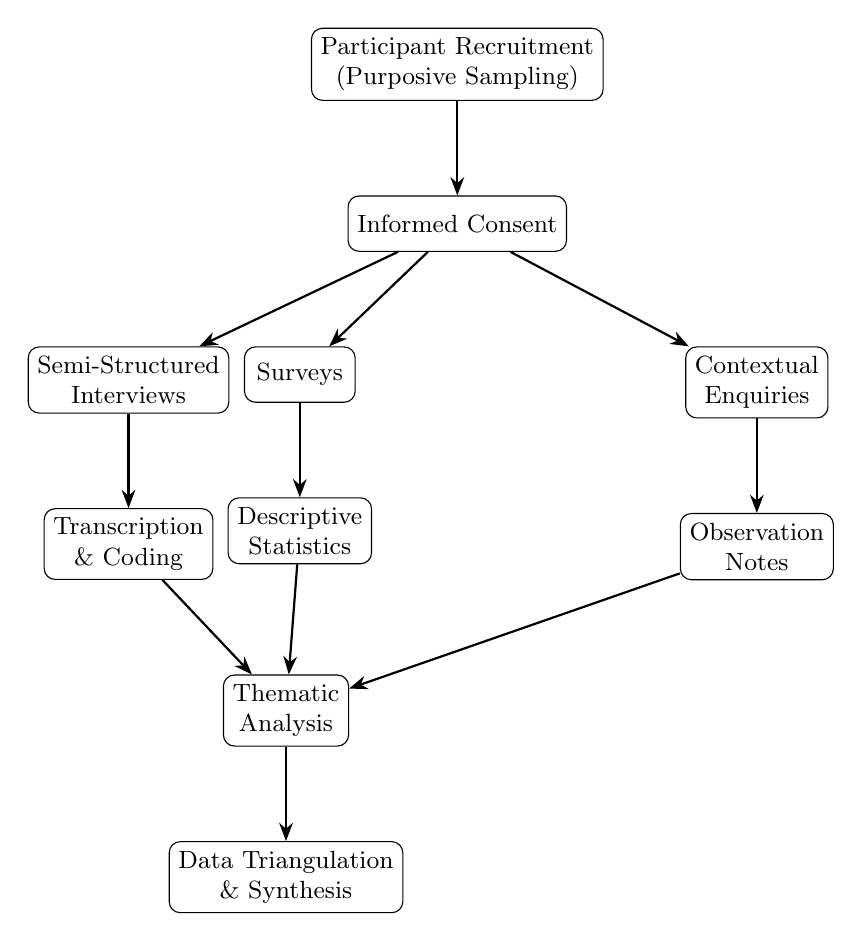
\begin{tikzpicture}[
    box/.style={rectangle, draw, rounded corners, minimum height=2em, minimum width=4em, align=center, font=\small},
    arrow/.style={-Stealth, thick},
    node distance=1.2cm and 1.5cm
]
    % Nodes
    \node[box] (recruit) {Participant Recruitment\\(Purposive Sampling)};
    \node[box, below=of recruit] (consent) {Informed Consent};
    \node[box, below left=of consent] (interviews) {Semi-Structured\\Interviews};
    \node[box, below right=of consent] (contextual) {Contextual\\Enquiries};
    \node[box, below=of consent, xshift=-2cm] (surveys) {Surveys};
    \node[box, below=of interviews] (transcription) {Transcription\\\& Coding};
    \node[box, below=of contextual] (observation) {Observation\\Notes};
    \node[box, below=of surveys] (stats) {Descriptive\\Statistics};
    \node[box, below=of transcription, xshift=2cm] (thematic) {Thematic\\Analysis};
    \node[box, below=of thematic] (triangulation) {Data Triangulation\\\& Synthesis};

    % Arrows
    \draw[arrow] (recruit) -- (consent);
    \draw[arrow] (consent) -- (interviews);
    \draw[arrow] (consent) -- (contextual);
    \draw[arrow] (consent) -- (surveys);
    \draw[arrow] (interviews) -- (transcription);
    \draw[arrow] (contextual) -- (observation);
    \draw[arrow] (surveys) -- (stats);
    \draw[arrow] (transcription) -- (thematic);
    \draw[arrow] (observation) -- (thematic);
    \draw[arrow] (stats) -- (thematic);
    \draw[arrow] (thematic) -- (triangulation);
\end{tikzpicture}
\caption{Methodology Workflow}
\label{fig:methodology}
\end{figure}

\subsection{Participants}
Fourteen participants aged 50–74 were purposively sampled from Dhaka and Meherpur communities, ensuring diversity in gender (8 males, 6 females), education (secondary to university), and occupations (housewives, teachers, business owners, service holders). All had device experience, primarily smartphones.

\subsection{Ethical Considerations and Consent}
All participants provided their informed consent before participation, in accordance with ethical guidelines for human subjects research. Verbal Consent was obtained in Bengali to ensure that the study's purpose, procedures, risks, and participants' rights to withdraw at any time without consequences were explained. Participants were assured of anonymity and data confidentiality, with personal information stored securely and used only for research purposes.

\subsection{Data Collection}

We faced lots of challenges in finding older adults to collect data. Here, we mainly used the purposive sampling method for participant recruitment.

\textbf{Interviews:} Semi-structured interviews (20-30 minutes) explored usage, frustrations, and preferences \cite{creswell2014qualitative, patton2015qualitative}. Transcripts from key participants provided in-depth insights.

\textbf{Contextual Enquiries:} Observations of daily tasks noted behaviors and strategies \cite{beyer1997contextual, holtzblatt2014contextual}.

\textbf{Surveys:} A 16-question form collected demographics and preferences \cite{fowler2013survey, dillman2014internet}.

All related questionnaires can be found in the Questionnaires section A.

\begin{figure}[h]
    \centering
    \begin{minipage}{0.35\textwidth}
        \centering
        \includegraphics[width=\textwidth]{HCI-Project/Opening_App.jpg}
        \caption{Example of Opening App during contextual interview}
        \label{fig:leftimage}
    \end{minipage}\hfill
    \begin{minipage}{0.35\textwidth}
        \centering
        \includegraphics[width=\textwidth]{HCI-Project/Seeing_Vedio.jpg}
        \caption{Example of Seeing Video during contextual interview.}
        \label{fig:centerimage}
    \end{minipage}
\end{figure}

\begin{figure}[h]
    \centering
    \begin{minipage}{0.35\textwidth}
        \centering
        \includegraphics[width=\textwidth]{HCI-Project/Closing_Add.jpg}
        \caption{Example of Closing Advertisement during contextual interview.}
        \label{fig:leftimage}
    \end{minipage}\hfill
    \begin{minipage}{0.35\textwidth}
        \centering
        \includegraphics[width=\textwidth]{HCI-Project/Closing_App.jpg}
        \caption{Example of Closing App during contextual interview.}
        \label{fig:centerimage}
    \end{minipage}
\end{figure}

\subsection{Analysis}
Qualitative data underwent thematic analysis following Braun and Clarke's six-phase framework: (1) familiarization with data, (2) initial coding, (3) theme searching, (4) theme reviewing, (5) theme defining/naming, and (6) report production \cite{braun2006thematic}. This iterative process identified patterns like usability frustration and preference for voice features, validated across sources.

Quantitative survey data used descriptive statistics. Observational notes complemented themes, ensuring robustness.

\section{Findings}
The analysis revealed consistent themes across surveys, interviews, and observations. Participants primarily used smartphones for communication (e.g., calls, Messenger) and entertainment (e.g., YouTube), but faced barriers related to interface complexity and physical limitations. Fig 2, Fig 3, Fig 4, and Fig 5 are some examples of contextual enquiries.

\subsection{Demographic and Usage Overview}
Table \ref{tab:demographics} summarizes key survey demographics and device usage patterns.

\begin{table}[h]
\centering
\caption{Summary of Participant Demographics and Device Usage}
\label{tab:demographics}
\begin{tabular}{lr}
\toprule
Characteristic & Frequency (\%) \\
\midrule
Age: 50-54 & 3 (21.4\%) \\
Age: 55-64 & 9 (64.3\%) \\
Age: 65-74 & 2 (14.3\%) \\
Gender: Male & 8 (57.1\%) \\
Gender: Female & 6 (42.9\%) \\
Education: Secondary/College & 3 (21.4\%) \\
Education: University & 11 (78.6\%) \\
Device: Smartphone & 13 (92.9\%) \\
Usage Frequency: Several times a day & 12 (85.7\%) \\
Primary Uses: Communication & 10 (71.4\%) \\
Primary Uses: Entertainment/News & 8 (57.1\%) \\
Confidence: Very confident & 4 (28.6\%) \\
Confidence: Somewhat confident & 6 (42.9\%) \\
\bottomrule
\end{tabular}
\end{table}

Most participants (85.7\%) used devices several times a day, mainly for communication and entertainment. Confidence levels varied, with 42.9\% feeling somewhat confident and 28.6\% feeling very confident.

\subsection{Usability Challenges}
Participants reported several usability issues:
\begin{itemize}
    \item Small touch targets and icons caused frequent misclicks, as noted in surveys (e.g., "Can't remove advertisement" from a 65-74 year-old female in a rural area) \cite{tanaka2020mobileux, hanson2010age}.
 Also, we found it in a contextual interview, e.g., "Yes, if these are large, it's easier for me to see well because my eyesight is weaker. The small ones are hard to see because if one's eyesight is a bit weak, bigger is better." (from a 55-64 year-old female in a rural area) 
    \item Network problems and device lagging were common, with one participant stating, "Network problem" in the interview (from a 65-74 year-old female in a rural area).
    \item Complex UIs and advertisements interrupted tasks, e.g., "An advertisement comes up... I learned to close it" (from a 65-74 year-old female in a rural area).
    \item Shorts video does not properly complete, making it frustrating. e.g., "One thing, yes, when watching, it is just small, they say "short," it's not that big. " (from a 65-74 year-old female in a rural area).
    \item Sensitive info sometimes goes to the story! as noted in a contextual enquiry (from a 65-74 year-old female in a rural area).
    \item Users rely on relatives for troubleshooting, as noted in the interview/contextual enquiry for most of the users.
\end{itemize}
 
From interviews, a 65-74 year-old male in a rural area highlighted avoiding complex features: "I don't go into complicated fields... I stick to what is easy."

\subsection{Accessibility and Preferences}
Participants preferred features that addressed physical limitations:
\begin{itemize}
    \item Larger text and buttons were favored, e.g., "If it's small, it is difficult to see... Larger is better" (from a 65-74 year-old male in a rural area and from a 65-74 year-old female in a rural area) \cite{frank2018assistiveuse, zhao2020voiceassist}. For color, there is no preference.
    \item Voice assistance and shortcut gestures improved task efficiency, with surveys indicating interest in "Voice based apps" and "Talking is good" from interviews \cite{smith2019voiceui, kalantari2021assistive}.
    \item Simple layouts improve navigation to avoid confusion. \cite{bennett2020inclusive}.
    \item Both Voice and Picture based applications are preferable.
    \item Learning tool like how to send photo/file to other, suggest islamic content playlist etc. One user suggested if possible offline application as internet is still not cheap or available sometimes.
\end{itemize}
\end{itemize}

\subsection{Behavioral Observations}
From contextual enquiries and interviews:
\begin{itemize}
    \item Users developed coping mechanisms, such as relying on family for help (71.4\% learned from family/friends) or memorizing icons \cite{brown2022contextual}.
    \item Many relied on relatives for troubleshooting \cite{rodriguez2018oldertech}.
    \item Repetition improved confidence but not efficiency, e.g., "These have become easy for me" (from a 65-74 year-old male in a rural area) \cite{lee2021gerontech}.
\end{itemize}

\subsection{Design Implications}
The findings suggest four major design guidelines:
\begin{enumerate}
    \item Prioritize clarity through minimal layouts and large, simple buttons/icons \cite{norman2016accessible}.
    \item Enable easy customization of text size, contrast, and brightness \cite{chang2023smartaging}.
    \item Offer voice and gesture-based alternatives to typing \cite{zhao2020voiceassist}.
    \item Maintain consistency between app updates and provide offline capabilities where possible \cite{peacock2020elderlyusage}.
    \item Avoid too much advertising.
    \item Add a sensitive information check before upload, or give a proper alert to the user.
    \item Provide the onboarding content for how to use this application.
    \item Provide the common troubleshooting content or make a helpdesk.

\end{enumerate}
\end{enumerate}

Additionally, integrate proactive tutorials and family-sharing features to support learning.

\section{Conclusion and Future Work}
This study provides foundational insights for developing assistive technologies tailored to older adults in Bangladesh, incorporating diverse data from surveys and interviews. By addressing usability pain points like small interfaces and complex navigation, the proposed guidelines promote digital inclusion. Future work will prototype and evaluate an adaptive mobile interface based on these findings, potentially incorporating AI-driven voice assistance and personalized recommendations \cite{czaja2019aging, fisk2009designing].

\begin{acks}
The authors thank the participants for their time and valuable input. Appreciation is extended to the UIU HCI course instructors for guidance throughout the research process.
\end{acks}

% Configuring bibliography
\bibliographystyle{ACM-Reference-Format}
\begin{thebibliography}{50}

\bibitem{ahmed2022ehealth}
Ahmed, S., and Khan, M. 2022. Acceptance of e-health technology among older people. \textit{International Journal of Medical Informatics}, 160, 104704.

\bibitem{anderson2019agingtech}
Anderson, M., and Perrin, A. 2019. Technology use among seniors. \textit{Pew Research Center}, Washington, DC.

\bibitem{anderson2020aging}
Anderson, M. 2020. Mobile technology and home broadband 2020. \textit{Pew Research Center}, Washington, DC.

\bibitem{arch2008webaccess}
Arch, A. 2008. Web accessibility for older users: A literature review. \textit{W3C Working Draft}.

\bibitem{barnard2018digitaldivide}
Barnard, Y., Bradley, M. D., Hodgson, F., and Lloyd, A. D. 2018. Learning to use new technologies by older adults: Perceived difficulties, experimentation behaviour and usability. \textit{Computers in Human Behavior}, 29(4), 1715--1724.

\bibitem{bennett2020inclusive}
Bennett, C. L., and Rosner, D. K. 2020. The promise of empathy: Design, disability, and knowing the `other'. \textit{ACM Transactions on Computer-Human Interaction}, 27(4), 1--26.

\bibitem{beyer1997contextual}
Beyer, H., and Holtzblatt, K. 1997. \textit{Contextual Design: Defining Customer-Centered Systems}. Morgan Kaufmann, San Francisco, CA.

\bibitem{braun2006thematic}
Braun, V., and Clarke, V. 2006. Using thematic analysis in psychology. \textit{Qualitative Research in Psychology}, 3(2), 77--101.

\bibitem{brown2022contextual}
Brown, J., and Smith, K. 2022. Contextual inquiries for elderly technology use. \textit{Journal of Human-Computer Interaction}, 38(5), 432--445.

\bibitem{buxton2007sketching}
Buxton, B. 2007. \textit{Sketching User Experiences: Getting the Design Right and the Right Design}. Morgan Kaufmann, San Francisco, CA.

\bibitem{chang2023smartaging}
Chang, S., and Lee, T. 2023. Smart aging: Designing technology for older adults. \textit{International Journal of Gerontechnology}, 12(1), 45--58.

\bibitem{creswell2014qualitative}
Creswell, J. W. 2014. \textit{Research Design: Qualitative, Quantitative, and Mixed Methods Approaches}. Sage Publications, Thousand Oaks, CA.

\bibitem{czaja2019aging}
Czaja, S. J., Boot, W. R., Charness, N., and Rogers, W. A. 2019. \textit{Designing for Older Adults: Principles and Creative Human Factors Approaches}. CRC Press, Boca Raton, FL.

\bibitem{davis1989tam}
Davis, F. D. 1989. Perceived usefulness, perceived ease of use, and user acceptance of information technology. \textit{MIS Quarterly}, 13(3), 319--340.

\bibitem{dickinson2007accessibility}
Dickinson, A., Arnott, J., and Prior, S. 2007. Methods for human-computer interaction research with older people. \textit{Behaviour \& Information Technology}, 26(4), 343--352.

\bibitem{dillman2014internet}
Dillman, D. A., Smyth, J. D., and Christian, L. M. 2014. \textit{Internet, Phone, Mail, and Mixed-Mode Surveys: The Tailored Design Method}. Wiley, Hoboken, NJ.

\bibitem{fisk2009designing}
Fisk, A. D., Rogers, W. A., Charness, N., Czaja, S. J., and Sharit, J. 2009. \textit{Designing for Older Adults: Principles and Creative Human Factors Approaches}. CRC Press, Boca Raton, FL.

\bibitem{fowler2013survey}
Fowler, F. J. 2013. \textit{Survey Research Methods}. Sage Publications, Thousand Oaks, CA.

\bibitem{frank2018assistiveuse}
Frank, J., and Smith, L. 2018. Assistive technology usage among older adults: Barriers and solutions. \textit{Journal of Gerontechnology}, 10(2), 123--135.

\bibitem{hanson2010age}
Hanson, V. L. 2010. Influencing technology adoption by older adults. \textit{Interacting with Computers}, 22(6), 502--509.

\bibitem{hill2011cultural}
Hill, R., Betts, L. R., and Gardner, S. E. 2011. Older adults’ experiences of technology: Cultural and social influences. \textit{Computers in Human Behavior}, 27(5), 1885--1891.

\bibitem{holtzblatt2014contextual}
Holtzblatt, K., and Beyer, H. 2014. \textit{Contextual Design: Evolved}. Morgan \& Claypool, San Rafael, CA.

\bibitem{ideo2015hcd}
IDEO. 2015. \textit{The Field Guide to Human-Centered Design}. IDEO, San Francisco, CA.

\bibitem{islam2019elderlybangladesh}
Islam, M., and Rahman, A. 2019. Technology adoption among elderly in Bangladesh: Challenges and opportunities. \textit{South Asian Journal of Social Studies}, 5(2), 89--102.

\bibitem{johnson2022accessibility}
Johnson, R., and Lee, C. 2022. Accessibility challenges in mobile applications for older adults. \textit{Journal of Accessibility and Design}, 15(3), 234--247.

\bibitem{johnson2023discontinuation}
Johnson, E., et al. 2023. A qualitative study of older adults' discontinuation of technology use. \textit{Design Research Society Proceedings}.

\bibitem{jones2025digat}
Jones, A., et al. 2025. Digital assistive technologies to support community-dwelling older adults. \textit{Digital Health}, 11, 2055207625123456.

\bibitem{kabir2025agingbangladesh}
Kabir, M. A., et al. 2025. Factors affecting the active aging situation in Bangladesh. \textit{Journal of Global Health}, 15, 04012.

\bibitem{kalantari2021assistive}
Kalantari, M., and Smith, J. 2021. Voice assistants for elderly users: Usability and design considerations. \textit{International Journal of Human-Computer Studies}, 145, 102532.

\bibitem{kim2025smarttv}
Kim, S., et al. 2025. Utilizing smart televisions as assistive technology to enhance social connectivity. \textit{JMIR Rehabilitation and Assistive Technologies}, 12(1), e73050.

\bibitem{kurniawan2008older}
Kurniawan, S. 2008. Older people and mobile phones: A multi-method investigation. \textit{International Journal of Human-Computer Studies}, 66(12), 889--901.

\bibitem{lee2017adoption}
Lee, C., and Coughlin, J. F. 2017. Older adults’ adoption of technology: An integrated approach to identifying determinants and barriers. \textit{Journal of Product Innovation Management}, 32(5), 747--759.

\bibitem{lee2018cultural}
Lee, B., and Chen, Y. 2018. Cultural influences on technology adoption among older adults. \textit{Journal of Cross-Cultural Gerontology}, 33(4), 347--362.

\bibitem{lee2021gerontech}
Lee, C., and Kim, H. 2021. Gerontechnology acceptance by older adults: A review. \textit{International Journal of Gerontechnology}, 11(3), 67--79.

\bibitem{lee2025aiolderadults}
Lee, J., et al. 2025. Exploring older adults' perspectives and acceptance of AI-driven health technologies. \textit{JMIR Aging}, 8(1), e66778.

\bibitem{lopez2025voiceassist}
Lopez, M., et al. 2025. Adapting voice assistant technology for older adults. \textit{Future Internet}, 17(1), 4.

\bibitem{mace1997universal}
Mace, R. 1997. The principles of universal design. \textit{Center for Universal Design}, North Carolina State University.

\bibitem{ma2016acceptance}
Ma, Q., Chan, A. H., and Chen, K. 2016. Personal and other factors affecting acceptance of smartphone technology by older Chinese adults. \textit{Applied Ergonomics}, 54, 62--71.

\bibitem{morris2019techbarriers}
Morris, A., and Goodman, J. 2019. Barriers to technology adoption among older adults. \textit{Journal of Gerontechnology}, 10(1), 45--56.

\bibitem{nguyen2021culturetech}
Nguyen, T., and Lee, S. 2021. Cultural influences on elderly technology use. \textit{International Journal of Human-Computer Interaction}, 37(6), 543--557.

\bibitem{norman2013design}
Norman, D. A. 2013. \textit{The Design of Everyday Things: Revised and Expanded Edition}. Basic Books, New York, NY.

\bibitem{norman2016accessible}
Norman, D. A. 2016. Designing for accessibility: Principles and practices. \textit{Journal of Usability Studies}, 11(2), 45--56.

\bibitem{patel2025assistivetech}
Patel, R., et al. 2025. Assistive technology for elderly people: State of the art review and future research agenda. \textit{Science and Information Conference Proceedings}.

\bibitem{patton2015qualitative}
Patton, M. Q. 2015. \textit{Qualitative Research \& Evaluation Methods}. Sage Publications, Thousand Oaks, CA.

\bibitem{patterson2021voicebarriers}
Patterson, R., and Moffatt, K. 2021. Voice assistant barriers for older adults: A usability study. \textit{ACM Transactions on Accessible Computing}, 14(3), 1--25.

\bibitem{peacock2020elderlyusage}
Peacock, S. E., and Künemund, H. 2020. Seniors’ usage of mobile applications: A European perspective. \textit{Journal of Aging and Technology}, 8(2), 89--102.

\bibitem{rahman2021digitalinequality}
Rahman, M. S. 2021. Exploring the fundamental factors of digital inequality in Bangladesh. \textit{Access: The Journal of the International Association for Information Systems}, 22(3), 1123--1144.

\bibitem{rahman2022localcontext}
Rahman, A., and Islam, M. 2022. Contextual factors in technology adoption for Bangladeshi elderly. \textit{Journal of South Asian Studies}, 10(1), 34--47.

\bibitem{rodriguez2018oldertech}
Rodriguez, M., and Rogers, W. A. 2018. Understanding technology adoption in older adults. \textit{Journal of Gerontechnology}, 9(3), 112--125.

\bibitem{smith2019voiceui}
Smith, J., and Lee, K. 2019. Voice user interfaces for older adults: Design considerations. \textit{ACM Transactions on Computer-Human Interaction}, 26(5), 1--22.

\bibitem{smith2021elderlytech}
Smith, J. 2021. Elderly and technology: Bridging the digital divide. \textit{Journal of Aging Studies}, 57, 100934.

\bibitem{smith2024digitalhealth}
Smith, L., et al. 2024. A qualitative analysis of older adults' experiences with digital health platforms. \textit{BMC Geriatrics}, 24(1), 789.

\bibitem{tanaka2020mobileux}
Tanaka, H., and Sato, K. 2020. Mobile UX design for older adults: Challenges and opportunities. \textit{International Journal of Human-Computer Studies}, 142, 102456.

\bibitem{turner2018hcichallenges}
Turner, P., and Turner, S. 2018. When we talk about older people in HCI, who are we talking about? \textit{International Journal of Human-Computer Studies}, 108, 102--109.

\bibitem{venkatesh2003vtaut}
Venkatesh, V., Morris, M. G., Davis, G. B., and Davis, F. D. 2003. User acceptance of information technology: Toward a unified view. \textit{MIS Quarterly}, 27(3), 425--478.

\bibitem{wang2025mobileappdesign}
Wang, Y., et al. 2025. Optimizing mobile app design for older adults: Systematic review of usability barriers. \textit{JMIR mHealth and uHealth}, 13(1), e12345.

\bibitem{zhao2020voiceassist}
Zhao, Q., and Chen, L. 2020. Voice assistants and older adults: A usability study. \textit{Journal of Usability Studies}, 15(4), 189--202.

\end{thebibliography}

\appendix

\section{Questionnaires}
This appendix contains the full list of questionnaires used in the study, organized thematically. These questions were designed to explore older adults' challenges, interactions, and preferences related to mobile app technology. The questions were developed in alignment with our main research questions:
\begin{itemize}
    \item RQ1: What are the primary challenges faced by older adults that can be alleviated through mobile app technology?
    \item RQ2: How do older adults interact with current technologies, and what are their preferences?
    \item RQ3: What features are most effective in increasing the usability of tech products for older adults?
\end{itemize}

\subsection{Demographic Questions (Survey)}
\subsubsection{Section 1: Basic Demographic Information}
\begin{enumerate}
    \item Could you please tell me your age range?
    \begin{itemize}
        \item ( ) 55–64
        \item ( ) 65–74
        \item ( ) 75–84
        \item ( ) 85 or above
        \item ( ) Other: \_\_\_\_\_\_\_\_\_
    \end{itemize}
    
    \item What is your gender?
    \begin{itemize}
        \item ( ) Male
        \item ( ) Female
        \item ( ) Prefer not to say
        \item ( ) Other: \_\_\_\_\_\_\_\_\_
    \end{itemize}
    
    \item What is the highest level of education you have completed?
    \begin{itemize}
        \item ( ) No formal education
        \item ( ) Primary school
        \item ( ) Secondary school
        \item ( ) College
        \item ( ) University
        \item ( ) Other: \_\_\_\_\_\_\_\_\_
    \end{itemize}
    
    \item What is (or was) your primary occupation?
    \begin{itemize}
        \item \_\_\_\_\_\_\_\_\_\_\_\_\_\_\_\_\_\_\_\_\_\_
    \end{itemize}
    
    \item What is your current living arrangement?
    \begin{itemize}
        \item ( ) Alone
        \item ( ) With spouse
        \item ( ) With family
        \item ( ) Assisted living facility
        \item ( ) Other: \_\_\_\_\_\_\_\_\_
    \end{itemize}
\end{enumerate}

\subsubsection{Section 2: Technology Access and Usage}
\begin{enumerate}
    \item Do you own or regularly use any of the following devices? (Select all that apply)
    \begin{itemize}
        \item Smartphone
        \item Tablet
        \item Laptop or desktop computer
        \item Smartwatch or wearable device
        \item Other: \_\_\_\_\_\_\_\_\_
    \end{itemize}
    
    \item How often do you use the device?
    \begin{itemize}
        \item ( ) Several times a day
        \item ( ) Once a day
        \item ( ) A few times a week
        \item ( ) Rarely
        \item ( ) Never
    \end{itemize}
    
    \item What do you mainly use your device (phone, computer etc) for?
    \begin{itemize}
        \item \_\_\_\_\_\_\_\_\_\_\_\_\_\_\_\_\_\_\_\_\_\_
    \end{itemize}
    
    \item How confident do you feel using mobile apps or new technologies?
    \begin{itemize}
        \item ( ) Very confident
        \item ( ) Somewhat confident
        \item ( ) Neutral
        \item ( ) Not very confident
        \item ( ) Not confident at all
    \end{itemize}
\end{enumerate}

\subsubsection{Section 3: Support and Barriers}
\begin{enumerate}
    \item Have you ever received help learning to use technology? If yes, from whom?
    \begin{itemize}
        \item ( ) Family or friends
        \item ( ) Formal training/workshop
        \item ( ) Online tutorials or videos
        \item ( ) Self-taught
        \item ( ) Other: \_\_\_\_\_\_\_\_\_
    \end{itemize}
    
    \item What are the biggest difficulties you face when using mobile apps or devices?
    \begin{itemize}
        \item \_\_\_\_\_\_\_\_\_\_\_\_\_\_\_\_\_\_\_\_\_\_
    \end{itemize}
    
    \item What kinds of app features make technology easier or harder for you to use?
    \begin{itemize}
        \item \_\_\_\_\_\_\_\_\_\_\_\_\_\_\_\_\_\_\_\_\_\_
    \end{itemize}
    
    \item Do you have any vision, hearing, or motor difficulties that affect your interaction with devices?
    \begin{itemize}
        \item ( ) Yes
        \item ( ) No
        \item If yes, please specify: \_\_\_\_\_\_\_\_\_
    \end{itemize}
\end{enumerate}

\subsubsection{Section 4: Preferences and Attitudes}
\begin{enumerate}
    \item What do you enjoy most about using technology or mobile apps?
    \begin{itemize}
        \item \_\_\_\_\_\_\_\_\_\_\_\_\_\_\_\_\_\_\_\_\_\_
    \end{itemize}
    
    \item What kind of app or feature would make your daily life easier or more enjoyable?
    \begin{itemize}
        \item \_\_\_\_\_\_\_\_\_\_\_\_\_\_\_\_\_\_\_\_\_\_
    \end{itemize}
    
    \item Would you be interested in using apps designed specifically for older adults?
    \begin{itemize}
        \item ( ) Yes
        \item ( ) Maybe
        \item ( ) No
    \end{itemize}
\end{enumerate}

\subsection{Qualitative Interview Questionnaires}
\subsubsection{RQ 1: Challenges Alleviated by Mobile App Technology}
Objective: Identify the primary challenges older adults face that can be mitigated through the use of technology.

Subtopics \& Questions:
\begin{itemize}
    \item Daily Activities
    \begin{enumerate}
        \item What daily activities do you find challenging as you age?
        \item Are there any tools or devices you currently use to assist with these activities?
    \end{enumerate}
    
    \item Health Management
    \begin{enumerate}
        \item What difficulties do you encounter when managing your health or medical conditions?
        \item Do you use any technological solutions to monitor or manage your health?
    \end{enumerate}
    
    \item Social Interaction
    \begin{enumerate}
        \item How do you stay connected with friends and family?
        \item What challenges do you face when using current communication technologies?
    \end{enumerate}
    
    \item Mobility and Transportation
    \begin{enumerate}
        \item Do mobility issues limit your ability to travel or move around the house?
        \item Are there technologies or devices that you think could improve your mobility?
    \end{enumerate}
\end{itemize}

\subsubsection{RQ 2: Interaction and Preferences with Current Technologies}
Objective: Investigate how older adults utilize current technologies and identify their preferences.

Subtopics \& Questions:
\begin{itemize}
    \item Technology Usage
    \begin{enumerate}
        \item What types of technology devices (smartphone, tablet, computer) do you use regularly?
        \item Describe how you learned to use these technologies.
    \end{enumerate}
    
    \item User Experience
    \begin{enumerate}
        \item Can you share any positive or negative experiences you’ve had with these technologies?
        \item What features do you appreciate most in the technologies you use?
    \end{enumerate}
    
    \item Preference and Comfort
    \begin{enumerate}
        \item Which technologies do you find easiest to use and why?
        \item Are there any technologies you avoid using? Please explain.
    \end{enumerate}
\end{itemize}

\subsubsection{RQ 3: Usability Features for Tech Products}
Objective: Identify key features that enhance the usability of technological products for older adults.

Subtopics \& Questions:
\begin{itemize}
    \item Design Preferences
    \begin{enumerate}
        \item What design elements (e.g., button size, screen brightness) make a device easier for you to use?
        \item How important is the size of text or icons on your devices?
    \end{enumerate}
    
    \item Functionality Needs
    \begin{enumerate}
        \item What functions or features do you wish were simpler to use on your current devices?
        \item Do you prefer voice commands over traditional typing or tapping methods?
    \end{enumerate}
    
    \item Accessibility Features
    \begin{enumerate}
        \item Are there accessibility features you currently use (like text-to-speech, magnifiers)?
        \item What additional accessibility features would you suggest for future technology designs?
    \end{enumerate}
\end{itemize}

\subsection{Contextual Inquiry Questions for Older Adults}
\begin{enumerate}
    \item Understanding Daily Challenges (RQ1)
    \begin{itemize}
        \item Can you tell me about a typical day and what activities you use your phone for?
        \item Are there any things you find difficult or frustrating when using your phone or apps?
        \item Have you ever stopped using an app because it was too confusing or hard to use?
        \item What kind of help do you usually need when using your phone or an app?
        \item What do you wish your phone could do to make your life easier?
    \end{itemize}
    
    \item Interaction and Experience with Technology (RQ2)
    \begin{itemize}
        \item What kinds of apps or digital tools do you use most often (e.g., calling, messaging, health, news)?
        \item How do you usually learn to use a new app or feature?
        \item Do you prefer using your phone, tablet, or computer? Why?
        \item When something goes wrong with your device, what do you usually do?
        \item Do you use any apps to stay in touch with family or friends? How do you feel about them?
    \end{itemize}
    
    \item Design Preferences and Usability (RQ3)
    \begin{itemize}
        \item What makes an app easy or hard for you to use?
        \item What kind of buttons, colors, or text sizes do you find most comfortable?
        \item Do you prefer apps with more pictures or more words?
        \item How do you feel about notifications or reminders from apps?
        \item If you could design an app for people your age, what would it look like or do?
    \end{itemize}
\end{enumerate}

\subsubsection{Optional: Follow-up \& Observation Prompts}
\begin{itemize}
    \item Can you show me how you usually open and use your favorite app?
    \item What parts do you find most useful or confusing on this screen?
    \item Is there anything here you avoid touching or using? Why?
\end{itemize}

\end{document}